\section{Metodología}
%\addcontentsline{toc}{chapter}{Diseño de la Solución}
%\setcounter{chapter}{2}
\pagenumbering{arabic}

% (Fernan y Johny)
% Está sección debe de contener:
% - Descripción detallada del flujo de trabajo
% - Preprocesamiento
% - Técnicas aplicadas
% - Herramientas utilizadas (Knime)
% - Parámetros claves
% - Métricas de Evaluación (Solo si aplica)

\subsection{Herramienta Utilizada: KNIME}

KNIME (Konstanz Information Miner) es una plataforma de código abierto diseñada para el análisis de datos, la minería de datos y el procesamiento de información mediante un entorno visual intuitivo. Esta herramienta permite construir flujos de trabajo (\textit{workflows}) de manera gráfica mediante la conexión de nodos predefinidos que realizan funciones específicas, lo cual facilita la integración, transformación y modelado de datos sin necesidad de escribir grandes bloques de código.

Una de las características más destacadas de KNIME es su arquitectura modular, que permite al usuario combinar múltiples técnicas analíticas, desde operaciones básicas de limpieza de datos hasta modelos avanzados de aprendizaje automático e inteligencia artificial. Además, KNIME ofrece compatibilidad con lenguajes de programación como Python y R, lo que amplía considerablemente su versatilidad y funcionalidad para usuarios avanzados.

En el contexto de este proyecto, KNIME se utiliza como herramienta central para el desarrollo de un flujo de trabajo de minería de texto, debido a su capacidad para integrar diversas tareas —como preprocesamiento, modelado de temas, minería de redes, análisis de sentimientos y muchos más— en un solo entorno visual. Esto no solo mejora la legibilidad del proceso, sino que también facilita la depuración, reutilización y documentación del flujo de trabajo.

Entre las ventajas clave de utilizar KNIME se encuentran:

\begin{description}
	\item[Interfaz visual intuitiva:] Permite diseñar flujos de trabajo mediante arrastrar y soltar, lo que reduce la curva de aprendizaje, especialmente para usuarios no expertos en programación.
	
	\item[Amplia biblioteca de nodos:] Cuenta con una gran cantidad de nodos preconfigurados para tareas comunes en minería de texto, aprendizaje automático y visualización de datos.
	
	\item[Extensibilidad:] Soporta la integración con lenguajes de programación como Python, R o Java, permitiendo personalizar operaciones complejas cuando sea necesario.
	
	\item[Reproducibilidad y colaboración:]  Los workflows pueden guardarse, compartirse y ejecutarse repetidamente, lo cual es fundamental para garantizar la reproducibilidad científica.
	
\end{description}


\subsection{Workflow de Ánalisis de Texto}

El siguiente \textit{workflow} en KNIME fue diseñado para realizar una serie de tareas relacionadas con la minería de texto para el problema presentando, incluyendo preprocesamiento, modelado de temas, minería de redes y análisis de sentimientos. La figura \ref{fig:knime_workflow} muestra la estructura completa del workflow, dividido en cuatro secciones principales: (1) Lectura y Preprocesamiento, (2) Modelado de Temas, (3) Minería de Redes y (4) Análisis de Sentimientos. A continuación, se describe cada componente y su función en detalle.

\begin{figure}[H]
	\centering
	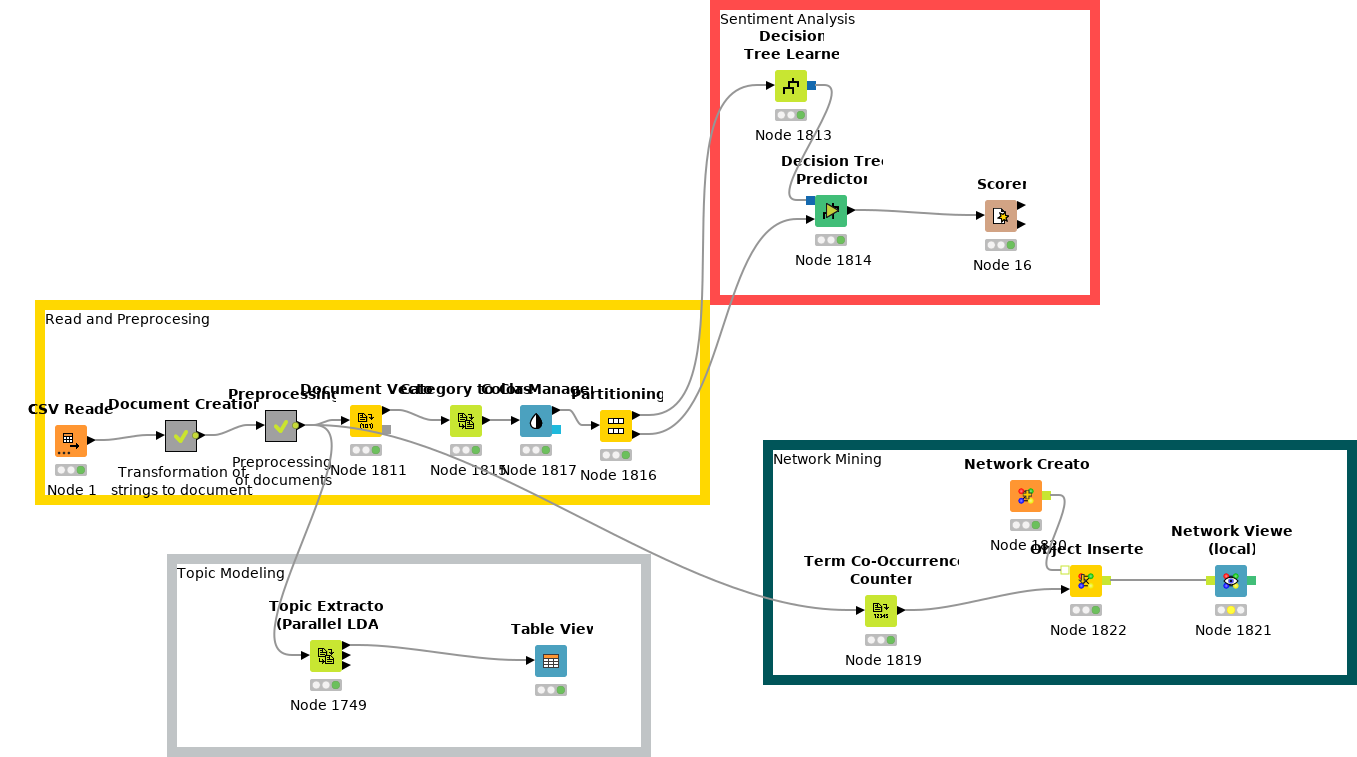
\includegraphics[width=\textwidth, height=0.8\textheight, keepaspectratio]{src/full_workflow.png}
	\caption{Workflow de KNIME para Minería de Texto}
	\label{fig:knime_workflow}
\end{figure}

\subsubsection{Lectura y Preprocesamiento}

La primera etapa del workflow está dedicada a la lectura de datos y el preprocesamiento inicial de los textos. Comienza con el nodo \textbf{CSV Reader}, que lee un archivo CSV que contiene los documentos de texto brutos. Este nodo es fundamental para cargar los datos iniciales en el flujo de trabajo.

Una vez cargados los datos, el metanodo \textbf{Document Creator} transforma las cadenas de texto brutas en objetos de documento estructurados, lo que facilita su procesamiento posterior. Este paso es crucial para preparar los datos para la aplicación de las técnicas posteriores. La figura \ref{fig:to_document} muestra el flujo utilizado para convertir a documento los textos

\begin{figure}[H]
	\centering
	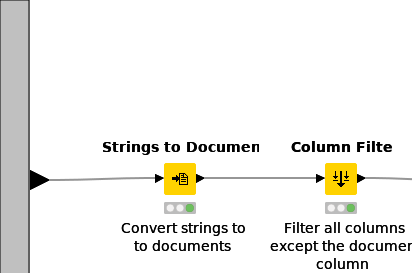
\includegraphics[width=\textwidth, height=0.8\textheight, keepaspectratio]{src/to_document}
	\caption[Flujo de conversión a Documento]{}
	\label{fig:to_document}
\end{figure}

El preprocesamiento es realizado por el metanodo \textit{preprocessing} y constituye una etapa crucial en la minería de texto, ya que mejora la calidad y la consistencia de los datos antes de aplicar técnicas avanzadas de análisis. En este workflow, el preprocesamiento se divide en varias fases, cada una de las cuales realiza una tarea específica. A continuación, se explica cada nodo y su función en detalle.

La figura \ref{fig:preprocessing_workflow} muestra el flujo de preprocesamiento utilizado en este proyecto.

\begin{figure}[H]
	\centering
	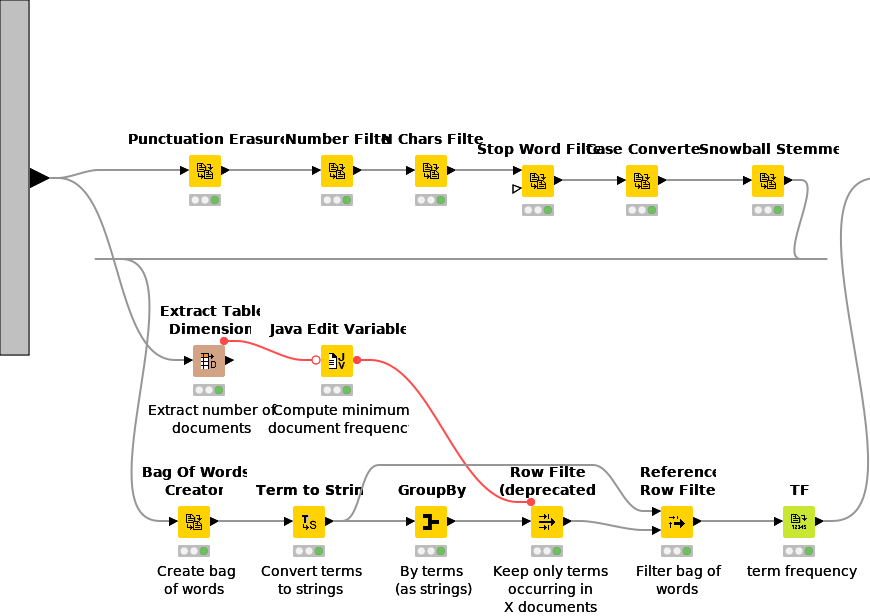
\includegraphics[width=\textwidth, height=0.8\textheight, keepaspectratio]{preprocessing.png}
	\caption[Flujo de Preprocesamiento en KNIME]{}
	\label{fig:preprocessing_workflow}
\end{figure}

El flujo de preprocesamiento descrito anteriormente fue diseñado teniendo en cuenta varios factores clave:

\begin{enumerate}
	\item \textbf{Reducción de Ruido: }La eliminación de stopwords, caracteres no alfanuméricos y la normalización de espacios en blanco ayudan a eliminar ruido del texto, lo que mejora la calidad de los datos de entrada.
	
	\item \textbf{Consistencia Lexical:} La conversión a minúsculas y la aplicación de stemming o lematización garantizan que las palabras similares se traten de manera consistente, reduciendo la dimensionalidad del vocabulario y mejorando la eficiencia del análisis.
	
	\item \textbf{Preparación para Modelos Avanzados:} Las operaciones de tokenización y creación de documentos estructurados preparan los datos para técnicas avanzadas de modelado, como el modelado de temas (LDA) y el análisis de sentimientos.
	
	\item \textbf{División de Datos:} La partición de los datos en conjuntos de entrenamiento y prueba es esencial para evaluar la efectividad del modelo de manera objetiva y evitar el sobreajuste.
\end{enumerate}

\subsubsection{Modelado de Temas}

En esta sección, el workflow utiliza técnicas de modelado de temas para identificar patrones temáticos en los documentos procesados.

Los resultados obtenidos del metanodo preprocesamiento alimenta al nodo \textbf{Topic Extractor (Parallel LDA)}, que implementa el algoritmo Latent Dirichlet Allocation (LDA) para extraer temas latentes en los documentos. Este modelo estima la distribución de temas en cada documento y la distribución de palabras en cada tema.

El nodo \textbf{Table View} proporciona una visualización tabular de los resultados del modelado de temas, permitiendo inspeccionar los temas generados y sus términos más relevantes.

\subsubsection{Minería de Redes}


La minería de redes se utiliza para analizar las interacciones y relaciones entre entidades extraídas de los documentos. Primero se construyen las relaciones con el nodo \textbf{Term Co-Occurrence Counter} calcula la frecuencia de co-ocurrencia de términos en los documentos, lo que permite capturar relaciones semánticas entre palabras El nodo \textbf{Network Creator (local)} construye una red basada en las relaciones detectadas durante el proceso de extracción de temas y co-ocurrencias de términos.

El nodo \textbf{Network Viewer} visualiza la red generada, permitiendo explorar las conexiones entre nodos y identificar clusters o comunidades significativas. Esta visualización es valiosa para comprender las estructuras subyacentes en los datos.

\subsubsection{Análisis de Sentimientos}

La última sección del workflow se centra en el análisis de sentimientos mediante aprendizaje automático. El nodo \textbf{Decision Tree Learner} entrena un modelo de árbol de decisión para clasificar los documentos según su polaridad (positiva, negativa o neutral). Este nodo utiliza características derivadas del preprocesamiento y el modelado de temas como entrada para el modelo.

El nodo \textbf{Decision Tree Predictor} aplica el modelo entrenado a nuevos datos para predecir la polaridad del sentimiento. Finalmente, el nodo \textbf{Scorer} evalúa la precisión del modelo comparando las predicciones con las etiquetas reales, proporcionando métricas de rendimiento como precisión, recall y F1-score.

\subsubsection{Flujo General del Workflow}

El workflow sigue un flujo lógico y secuencial:
\begin{enumerate}
	\item Los datos se leen y preprocesan para prepararlos para el análisis.
	
	\item Se extraen temas latentes utilizando LDA para identificar patrones temáticos.
	
	\item Se construye y visualiza una red basada en las relaciones entre términos y documentos.
	
	\item Se realiza un análisis de sentimientos utilizando un modelo de árbol de decisión para clasificar la polaridad de los textos.
\end{enumerate}

Este enfoque integrado permite abordar múltiples aspectos de la minería de texto, desde la extracción de conocimiento hasta la interpretación de emociones y relaciones.



